\subsection{Decimo sprint}

\begin{minipage}{\textwidth}
  Di seguito è riportata la distribuzione delle ore per ciascun membro del team, accumulate in totali per persona e per ruolo:
  \begin{table}[H]
    \begin{tabularx}{\textwidth}{|c|*{6}{>{\centering}X|}c|}
      \hline
      \multicolumn{8}{|c|}{\textbf{Consuntivo orario}} \\
      \hline
      \textbf{Membro del team} & \textbf{Re} & \textbf{Am} & \textbf{An} & \textbf{Pt} & \textbf{Pr} & \textbf{Ve} & \textbf{Totale per persona} \\
      \hline
      Cavalli Riccardo & 0 & 0 & 0 & 5 & 1 & 3 & 9 \\
      \hline
      Pianon Raul & 0 & 0 & 0 & 6 & 1 & 2 & 9 \\
      \hline
      Dall’Amico Martina & 0 & 0 & 0 & 2 & 6 & 1 & 9 \\
      \hline
      Cristo Marco & 1 & 0 & 0 & 6 & 0 & 2 & 9 \\
      \hline
      Lewental Sebastiano & 1 & 1 & 0 & 4 & 0 & 3 & 9 \\
      \hline
      Zecchinato Mattia & 0 & 0 & 1 & 0 & 5 & 3 & 9 \\
      \hline
      Stocco Tommaso & 2 & 0 & 0 & 4 & 0 & 3 & 9 \\
      \hline
      \textbf{Totale ore per ruolo} & 4 & 1 & 1 & 27 & 13 & 17 & \textbf{63} \\
      \hline
    \end{tabularx}
    \caption{Sprint 10 - Consuntivo orario}
  \end{table}
  \end{minipage}

  \begin{figure}[H]
    \centering
    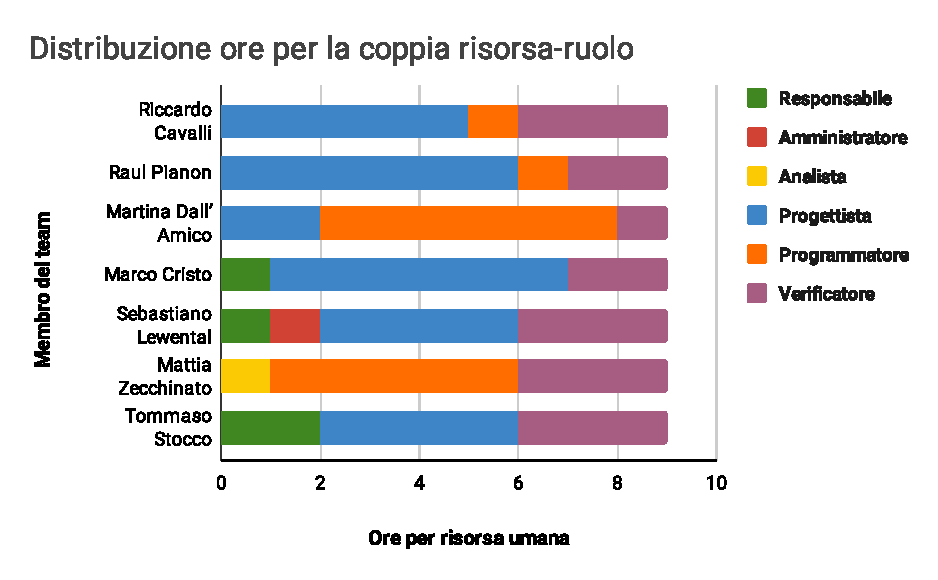
\includegraphics[width=0.90\textwidth]{assets/Consuntivo/Sprint-10/distribuzione_ore_risorsa_ruolo.pdf}
    \caption{Sprint 10 - Istogramma della distribuzione oraria per la coppia risorsa-ruolo}
  \end{figure}

  \begin{figure}[H]
    \centering
    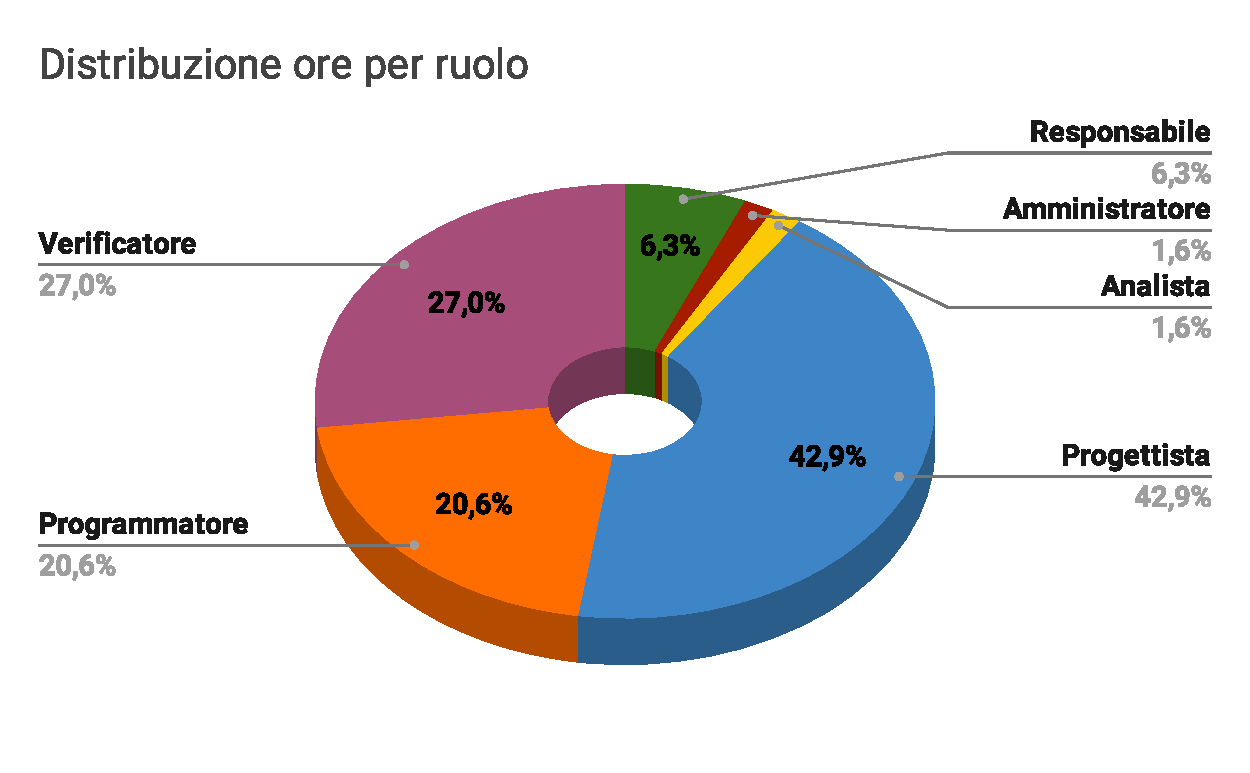
\includegraphics[width=0.90\textwidth]{assets/Consuntivo/Sprint-10/distribuzione_ore_ruolo.pdf}
    \caption{Sprint 10 - Areogramma della distribuzione oraria per ruolo}
  \end{figure}

  \begin{minipage}{\textwidth}
  Di seguito è riportato il consuntivo economico del decimo \glossario{sprint}:
  \begin{table}[H]
  \begin{adjustwidth}{-0.5cm}{-0.5cm}
    \centering
    \begin{tabular}{|P{2.9cm}|P{2.3cm}|P{2.5cm}|P{2.3cm}|>{\arraybackslash}P{2.5cm}|}
      \hline
      \multicolumn{5}{|c|}{\textbf{Consuntivo economico}} \\
      \hline
      \textbf{Ruolo} & \textbf{Ore per ruolo} & \textbf{Delta ore preventivo - consuntivo} & \textbf{Costo (in \texteuro)} & \textbf{Delta costo preventivo - consuntivo (in \texteuro)} \\
      \hline
      \Responsabile[U]{} & 4 & 0 & 120,00 & 0,00 \\ \hline
      \Amministratore[U]{} & 1 & 1 & 20,00 & 20,00 \\ \hline
      \Analista[U]{} & 1 & 0 & 25,00 & 0,00 \\ \hline
      \Progettista[U]{} & 27 & 3 & 675,00 & 75,00 \\ \hline
      \Programmatore[U]{} & 13 & -2 & 195,00 & -30,00 \\ \hline
      \Verificatore[U]{} & 17 & -1 & 255,00 & -15,00 \\ \hline
      \textbf{Totale} & \textbf{63} & 1 & \textbf{1290,00} & 50,00 \\ \hline
      \textbf{Restante} & 219 & / & 4.420,00 & / \\ \hline
      \textbf{Sprint pregressi} & 364 & / & 7.310,00 & / \\ \hline
    \end{tabular}
    \caption{Sprint 10 - Consuntivo economico}
  \end{adjustwidth}
  \end{table}
  \end{minipage}

  \begin{figure}[H]
    \centering
    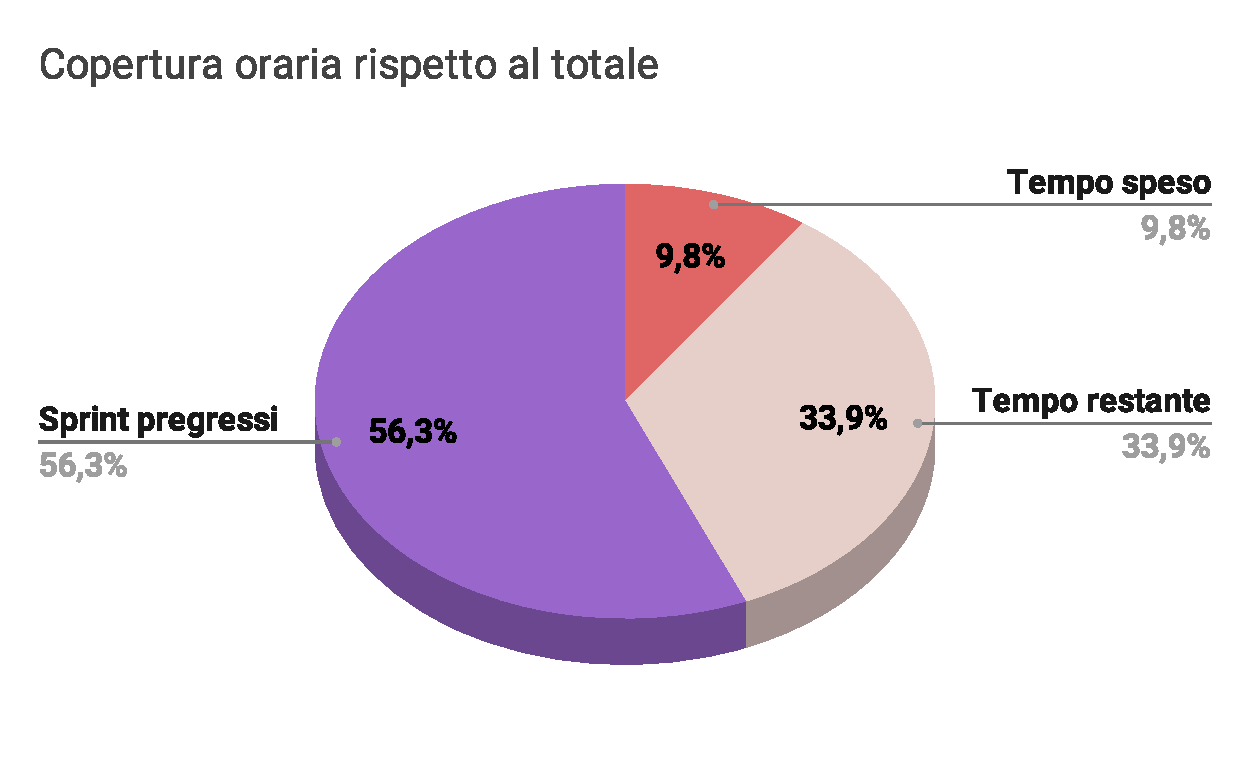
\includegraphics[width=0.90\textwidth]{assets/Consuntivo/Sprint-10/copertura_oraria.pdf}
    \caption{Sprint 10 - Areogramma del tempo speso (in ore) rispetto al totale}
  \end{figure}

  \begin{figure}[H]
    \centering
    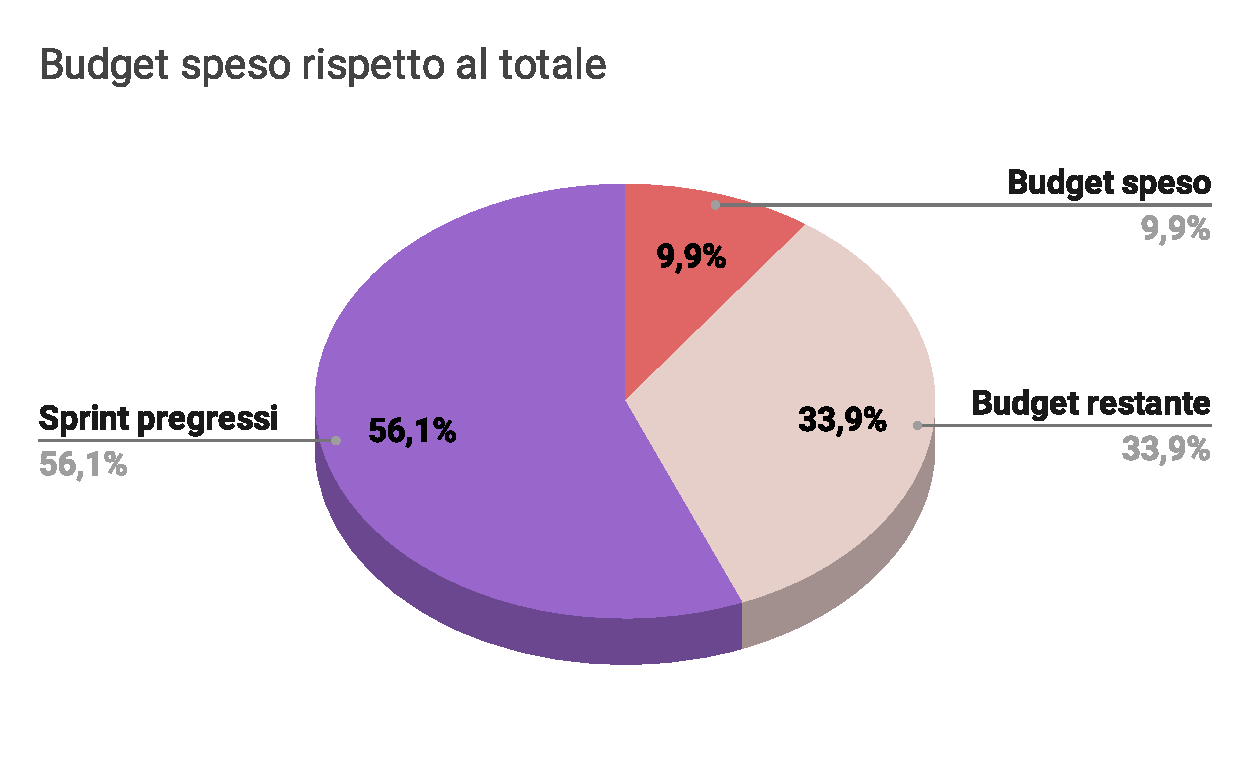
\includegraphics[width=0.90\textwidth]{assets/Consuntivo/Sprint-10/budget_speso.pdf}
    \caption{Sprint 10 - Areogramma del budget speso rispetto al totale}
  \end{figure}

  \begin{minipage}{\textwidth}
    Di seguito sono riportate le ore rimanenti per la coppia risorsa-ruolo:
    \begin{table}[H]
      \begin{tabularx}{\textwidth}{|c|*{6}{>{\centering}X|}c|}
        \hline
        \multicolumn{8}{|c|}{\textbf{Ore rimanenti per la coppia risorsa-ruolo}} \\
        \hline
        \textbf{Membro del team} & \textbf{Re} & \textbf{Am} & \textbf{An} & \textbf{Pt} & \textbf{Pr} & \textbf{Ve} & \textbf{Totale per persona} \\
        \hline
        Cavalli Riccardo & 0 & 0 & 3 & 7 & 9 & 6 & 25 \\
        \hline
        Pianon Raul & 2 & 1 & 1 & 13 & 8 & 4 & 29 \\
        \hline
        Dall’Amico Martina & 2 & 1 & 1 & 12 & 10 & 7 & 33 \\
        \hline
        Cristo Marco & 1 & 4 & 0 & 11 & 10 & 5 & 31 \\
        \hline
        Lewental Sebastiano & 2 & 3 & 1 & 7 & 11 & 8 & 32 \\
        \hline
        Zecchinato Mattia & 5 & 2 & 2 & 9 & 6 & 8 & 32 \\
        \hline
        Stocco Tommaso & 3 & 0 & 3 & 15 & 9 & 5 & 35 \\
        \hline
        \textbf{Totale ore per ruolo} & 15 & 12 & 11 & 74 & 64 & 43 & \textbf{219} \\
        \hline
      \end{tabularx}
      \caption{Sprint 10 - Ore rimanenti per la coppia risorsa-ruolo}
    \end{table}
  \end{minipage}

\subsubsection{Revisione delle attività}

Nell'arco del decimo \glossario{sprint}, il team ha svolto le seguenti attività:
\begin{itemize}
 \item Verifica e rilascio dei seguenti documenti:
  \begin{itemize}
    \item \NdP;
    \item \PdP;
    \item \AdR{} (post colloquio \RTB);
    \item \PdQ.
  \end{itemize}
  \item Correzioni alla documentazione post revisione \glossario{RTB};
  \item Stesura verbali interni;
  \item Aggiornamento dei grafici nel \PdQ;
  \item Miglioramento e formalizzazione delle convenzioni per lo stile di codifica;
  \item Progettazione architetturale \glossario{front-end};
  \item Progettazione logica \glossario{back-end};
  \item Modifica della struttura del front-end;
  \item Valutazione di possibili architetture per il back-end;
  \item Stesura di una relazione sulle architetture individuate;
  \item Progettazione di dettaglio front-end;
  \item Progettazione del database;
  \item Definizione di nuovi \glossario{dizionari dati};
  \item Selezione degli strumenti di test;
  \item Sperimentazione dei test di unità con pytest e Jest;
  \item Codifica e test di unità front-end;
  \item Configurazione di strumenti di formattazione e \glossario{linting} del codice;
  \item Stesura del documento \ST;
  \item Stesura del \MU\ (sezioni riguardanti la chat, la gestione dei dizionari e la configurazione delle impostazioni);
  \item Aggiornamento del file \textit{README} e dei requisiti di sistema;
  \item Utilizzo di \glossario{SonarLint} per il calcolo della complessità dei metodi.
\end{itemize}

\subsubsection{Retrospettiva}

\par Di seguito sono riportati i risultati del questionario di valutazione dello \glossario{sprint}:
\begin{itemize}
  \item Organizzazione dello \glossario{sprint}\ - Valutazione: 8;
  \item Conduzione dei meeting interni - Valutazione: 8.5;
  \item Impegno e partecipazione dei singoli membri - Valutazione: 7;
  \item Tutti i membri del team erano a conoscenza delle proprie mansioni;
  \item La numerosità delle riunioni è risultata adeguata per quasi tutti i membri del gruppo;
  \item Le riunioni sono state organizzate quasi sempre con il giusto preavviso;
  \item Il rapporto ore spese/ore produttive e la produttività generale sono migliorati rispetto agli sprint precedenti.
\end{itemize}

\vspace{0.5\baselineskip}
\par A seguire le \textbf{analisi a posteriori} del decimo \glossario{sprint}:
\begin{itemize}
  \item Il gruppo ha superato con successo la revisione \glossario{RTB}, dimostrando una solida comprensione degli obiettivi del capitolato e delle tecnologie necessarie per conseguirli;
  \item Durante la fase centrale dello sprint, il monitoraggio delle attività è stato meno costante rispetto al resto del periodo. Poiché il team ha deciso di tornare alla formula di sprint di due settimane, è necessario un controllo continuo da parte del responsabile;
  \item La progettazione del \glossario{back-end} ha comportato una fase iniziale di valutazione delle architetture potenziali. Questo ha causato un rallentamento nelle attività di progettazione e codifica;
  \item Il team di progettisti ha lavorato alla ristrutturazione del \glossario{front-end}, conseguendo una significativa riduzione della complessità dei metodi e delle funzioni;
  \item Il gruppo ha configurato strumenti per formattare automaticamente il codice prima di ogni commit. Questa configurazione riduce le problematiche legate al caricamento e all'estrazione del codice dal \glossario{repository} remoto;
  \item Inoltre, sono stati configurati strumenti di linting per eseguire un'analisi statica del codice prima di ogni commit;
  \item L'amministratore ha incontrato difficoltà nel reperire strumenti per il calcolo automatico delle metriche di qualità del codice. A partire dal prossimo sprint, verranno allocate più risorse per affrontare questa attività;
  \item Il team ha incrementato l'efficienza di merge delle pull request, stabilendo un ritmo soddisfacente per la verifica, approvazione e integrazione delle modifiche;
  \item Il gruppo ha configurato l'ambiente di test per il back-end e il front-end. In vista del prossimo sprint, l'obiettivo è definire un workflow su \glossario{GitHub} che garantisca la conformità del codice caricato nel repository agli standard previsti.
\end{itemize}

\subsubsection{Aggiornamento pianificazione e preventivo}
\par Il team ha definito un piano d'azione per migliorare l'organizzazione e la produttività del prossimo \glossario{sprint}:
\begin{itemize}
  \item Pianificare gli incontri con almeno un giorno di anticipo;
  \item Lavorare in team di due o più persone per le attività di progettazione, codifica e testing;
  \item Maggior focus e allocazione di risorse per la progettazione e codifica \glossario{back-end};
  \item Individuazione di strumenti per il calcolo automatico delle metriche di qualità del codice.
\end{itemize}

\paragraph*{Pianificazione futura:}
\par Nel corso dello \glossario{sprint}, il team si è concentrato sulla progettazione del \glossario{front-end}, che ha raggiunto un buon livello di dettaglio. Inoltre, il gruppo ha compiuto significativi progressi nella codifica del front-end. Per quanto riguarda il \glossario{back-end}, il team ha progettato il \glossario{database} e scelto il modello architetturale da seguire. Di conseguenza, il prossimo sprint sarà dedicato alla progettazione di dettaglio e alla codifica del back-end.

\par Durante lo sprint appena concluso, il gruppo ha definito ulteriori convenzioni per lo stile di codifica, che saranno formalizzate nelle \NdP\ nel prossimo sprint. Inoltre, verranno progettati i test di unità e saranno eseguiti test manuali utilizzando database locali e \glossario{dizionari dati} complessi.

\paragraph*{Preventivo "a finire" (\sezione{sec:stima_temporale}):}
\par Come illustrato nella \sezione{sec:preventivo-a-finire}, le ore riportate nel preventivo "a finire" sono equamente distribuite tra i membri del team. La maggior parte delle ore è assegnata ai ruoli di progettista, programmatore e verificatore; pertanto, il gruppo non ha ritenuto necessaria una ridistribuzione delle ore. Il team prevede di rispettare il budget preventivato e di completare il progetto entro la data di consegna prevista per metà settembre.

\paragraph*{Gestione dei rischi (\sezione{sec:analisi_rischi}):}
\par Durante il decimo \glossario{sprint}, i seguenti rischi sono stati gestiti con successo:
\begin{itemize}
  \item \textbf{RT3 - Malfunzionamenti software}: il gruppo ha riscontrato degli errori durante la costruzione delle immagini \glossario{Docker}. Inoltre, sono state eseguite attività di configurazione e refactoring che hanno generato malfunzionamenti software. Queste attività includono:
  \begin{itemize}
    \item Configurazione di strumenti per la formattazione e il \glossario{linting} del codice;
    \item Impostazione di software per la generazione automatica della documentazione;
    \item Creazione di funzioni componibili con \glossario{Vue.js};
    \item Configurazione degli strumenti di test.
  \end{itemize}
  Nonostante la complessità di alcuni errori, il team ha prontamente risolto i problemi attraverso l'apertura di ticket e discussioni nelle apposite sezioni di \glossario{GitHub}. Quando necessario, sono stati organizzati incontri specifici per la risoluzione tempestiva di bug e malfunzionamenti.
\end{itemize}